\section{Virtual CED}
\label{sec:chapter_4_section_2}
Il progetto di modellazione di un Virtual CED (Centro Elaborazione Dati) sviluppato presso SOGEI, \`e stato realizzato con
l'intento di avere un modello 3D navigabile per consentire di sviluppare un sistema di Indoor Mapping e Indoor Navigation.
Sono stati sviluppati dei plugins coerenti con il contesto, di seguito come si vede in Figura~\ref{fig:virtualCED}) una
vista 3D del modello dall'alto.\\

\begin{figure}[htbp] %  figure placement: here, top, bottom, or page
   \centering
   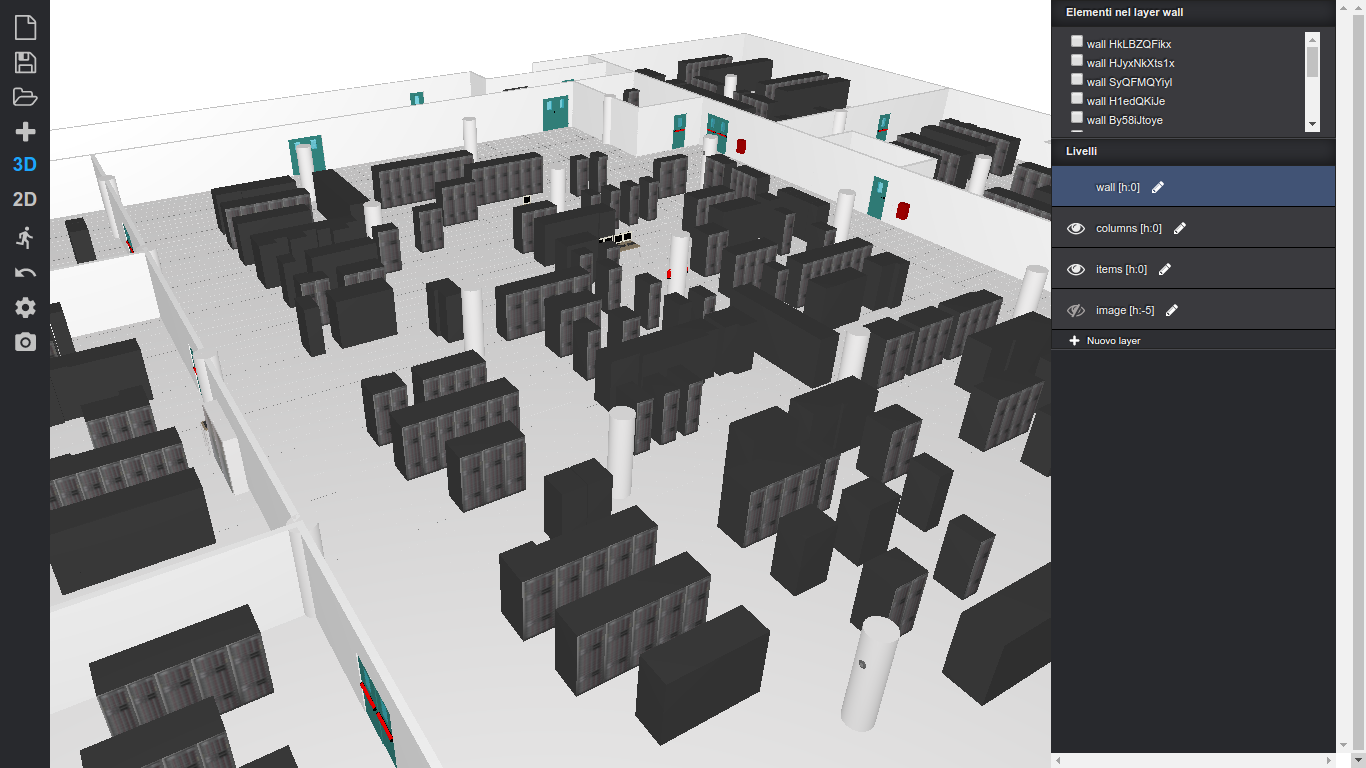
\includegraphics[width=1\linewidth]{images/virtualCED}
   \caption{Vista 3D di un Virtual CED}
   \label{fig:virtualCED}
   \end{figure}

\newpage
Il primo gruppo di \emph{Plugin} sono riguardano il contesto della sicurezza degli edifici, come
si vede in Figura~\ref{fig:figura6} essi sono: un estintore, un rilevatore di fumo, una cassetta naspo ed una
porta antipanico.
\begin{figure}[htbp]
\begin{center}
\begin{tabular}{c @{\hspace{1em}} c}
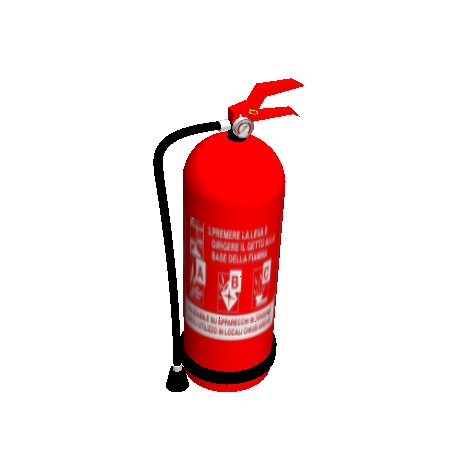
\includegraphics[width=5.5cm]{images/estintore} &
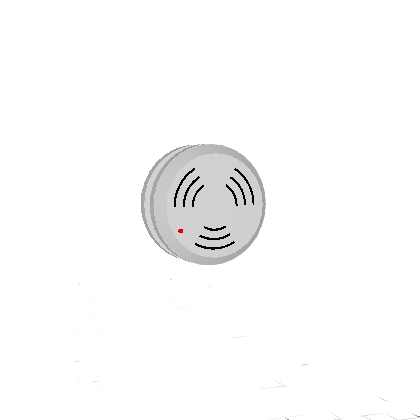
\includegraphics[width=5.5cm]{images/rilevatore} \\
 (a) & (b) \\
\end{tabular}
\begin{tabular}{c @{\hspace{1em}} c}
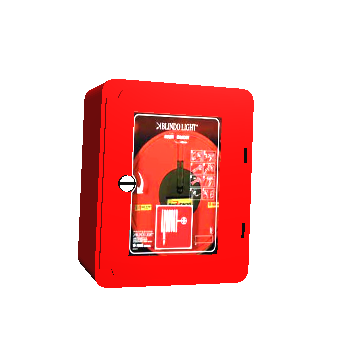
\includegraphics[width=5.5cm]{images/naspo} &
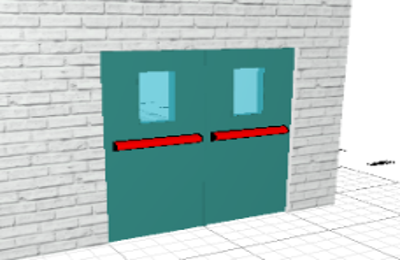
\includegraphics[width=5.5cm]{images/panicDoorDouble} \\
 (c) & (d) \\
\end{tabular}
\end{center}
\caption{Dettaglio Plugins: (a) estintore, (b) rilevatore fumo, (c) naspo, (d) porta antipanico}\label{fig:figura6}
\end{figure}
\newpage

Il secondo gruppo di \emph{Plugin} riguardano il contesto tecnologico (Figura~\ref{fig:figura7}), essi sono
un metal detector, un rack server, un router wifi ed una telecamera. Questo gruppo ha un importanza rilevate in quanto
essi possono consentire un accesso remoto ed essere considerati dispositivi \emph{IoT}.\\
\begin{figure}[htbp]
\begin{center}
\begin{tabular}{c @{\hspace{1em}} c}
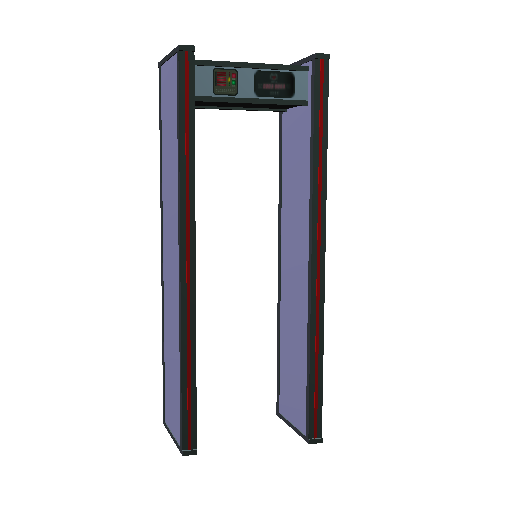
\includegraphics[width=5.5cm]{images/metalDetector} &
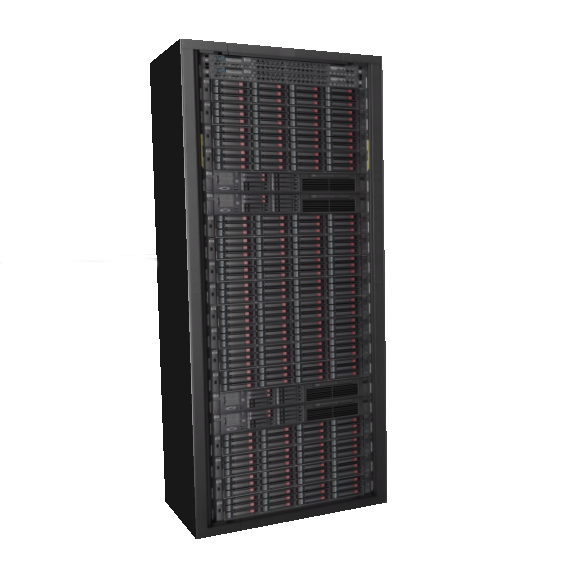
\includegraphics[width=5.5cm]{images/rack} \\
 (a) & (b) \\
\end{tabular}
\begin{tabular}{c @{\hspace{1em}} c}
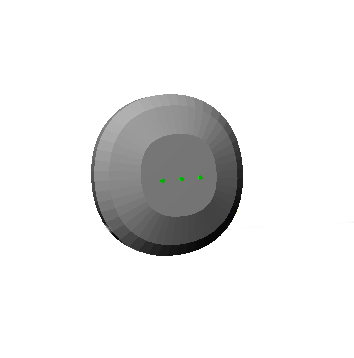
\includegraphics[width=5.5cm]{images/routerWifi} &
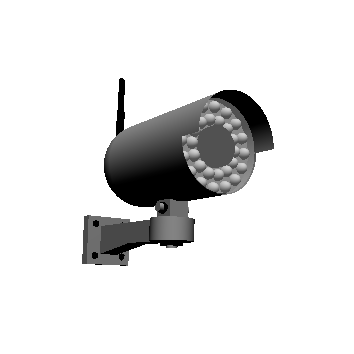
\includegraphics[width=5.5cm]{images/telecamera} \\
 (c) & (d) \\
\end{tabular}
\end{center}
\caption{Dettaglio Plugin: (a) metal detector, (b) rack server, (c) router wifi, (d) telecamera}\label{fig:figura7}
\end{figure}
